\section{Objetivos}
\begin{itemize}
    \item Determinar las líneas de campo de diferentes imanes para visualizar y entender la influencia magnética que ejercen en su entorno.
    \item Desarrollar una comprensión de la medición del campo magnético, familiarizándose con sus unidades y métodos de medición en diferentes configuraciones.
    \item Diferenciar entre diversos tipos de imanes y explorar sus aplicaciones prácticas en tecnología y dispositivos cotidianos.
    \item Determinar experimentalmente el campo magnético terrestre en el laboratorio, aplicando conceptos teóricos y técnicas de medición directa.
\end{itemize}

\section{Marco Teórico}
Los imanes son fundamentales en numerosas aplicaciones tecnológicas, desde la generación de electricidad hasta el almacenamiento de datos. Estos objetos ejercen fuerzas sobre materiales ferromagnéticos y otros imanes, un fenómeno que se debe a sus campos magnéticos, los cuales son regiones espaciales influenciadas por las propiedades magnéticas de los imanes.

\subsection{Naturaleza de los Imanes}
Descubiertos históricamente en la forma de magnetita, los imanes permanentes como el hierro, el níquel y el cobalto, poseen polos norte y sur, donde el campo magnético es más intenso. La interacción entre estos polos sigue reglas específicas: polos iguales se repelen y polos opuestos se atraen. Esta propiedad es invariable; al dividir un imán, cada fragmento siempre contará con ambos polos.

\subsection{Campo Magnético Terrestre}
La Tierra misma es un imán gigante con un campo magnético que interactúa con los imanes locales y afecta a brújulas y otros dispositivos de navegación. Este laboratorio busca medir y entender tanto los campos magnéticos generados por imanes artificiales como el campo magnético terrestre.

\subsection{Campo Magnético de las Bobinas de Helmholtz}
Se utilizarán bobinas de Helmholtz para generar un campo magnético controlable y medir su interacción con el campo terrestre. Estas bobinas permiten crear un campo magnético homogéneo que se puede ajustar mediante cambios en la corriente eléctrica suministrada, lo que es crucial para estudios precisos de campos magnéticos.

La comprensión y aplicación de estos conceptos permite no solo apreciar cómo funcionan los dispositivos basados en el magnetismo, sino también desarrollar nuevas aplicaciones y mejorar las tecnologías existentes.

\section{Análisis y discusión: Montaje 1 Imanes}

\subsection{Determine las líneas de campo con imanes}
\textbf{Con las limaduras de hierro determine las líneas de campo de los diferentes imanes,
describa lo que observa}
Al esparcir limaduras de hierro sobre una lámina de vidrio con diferentes imanes dispuestos debajo, se pudo observar claramente la forma y dirección de las líneas de campo magnético. En cada caso, las limaduras se alinearon formando patrones que delinean las líneas de campo emanadas desde los polos de los imanes.

\begin{figure}[H]
  \centering
  \begin{minipage}{0.45\textwidth}
    \centering
    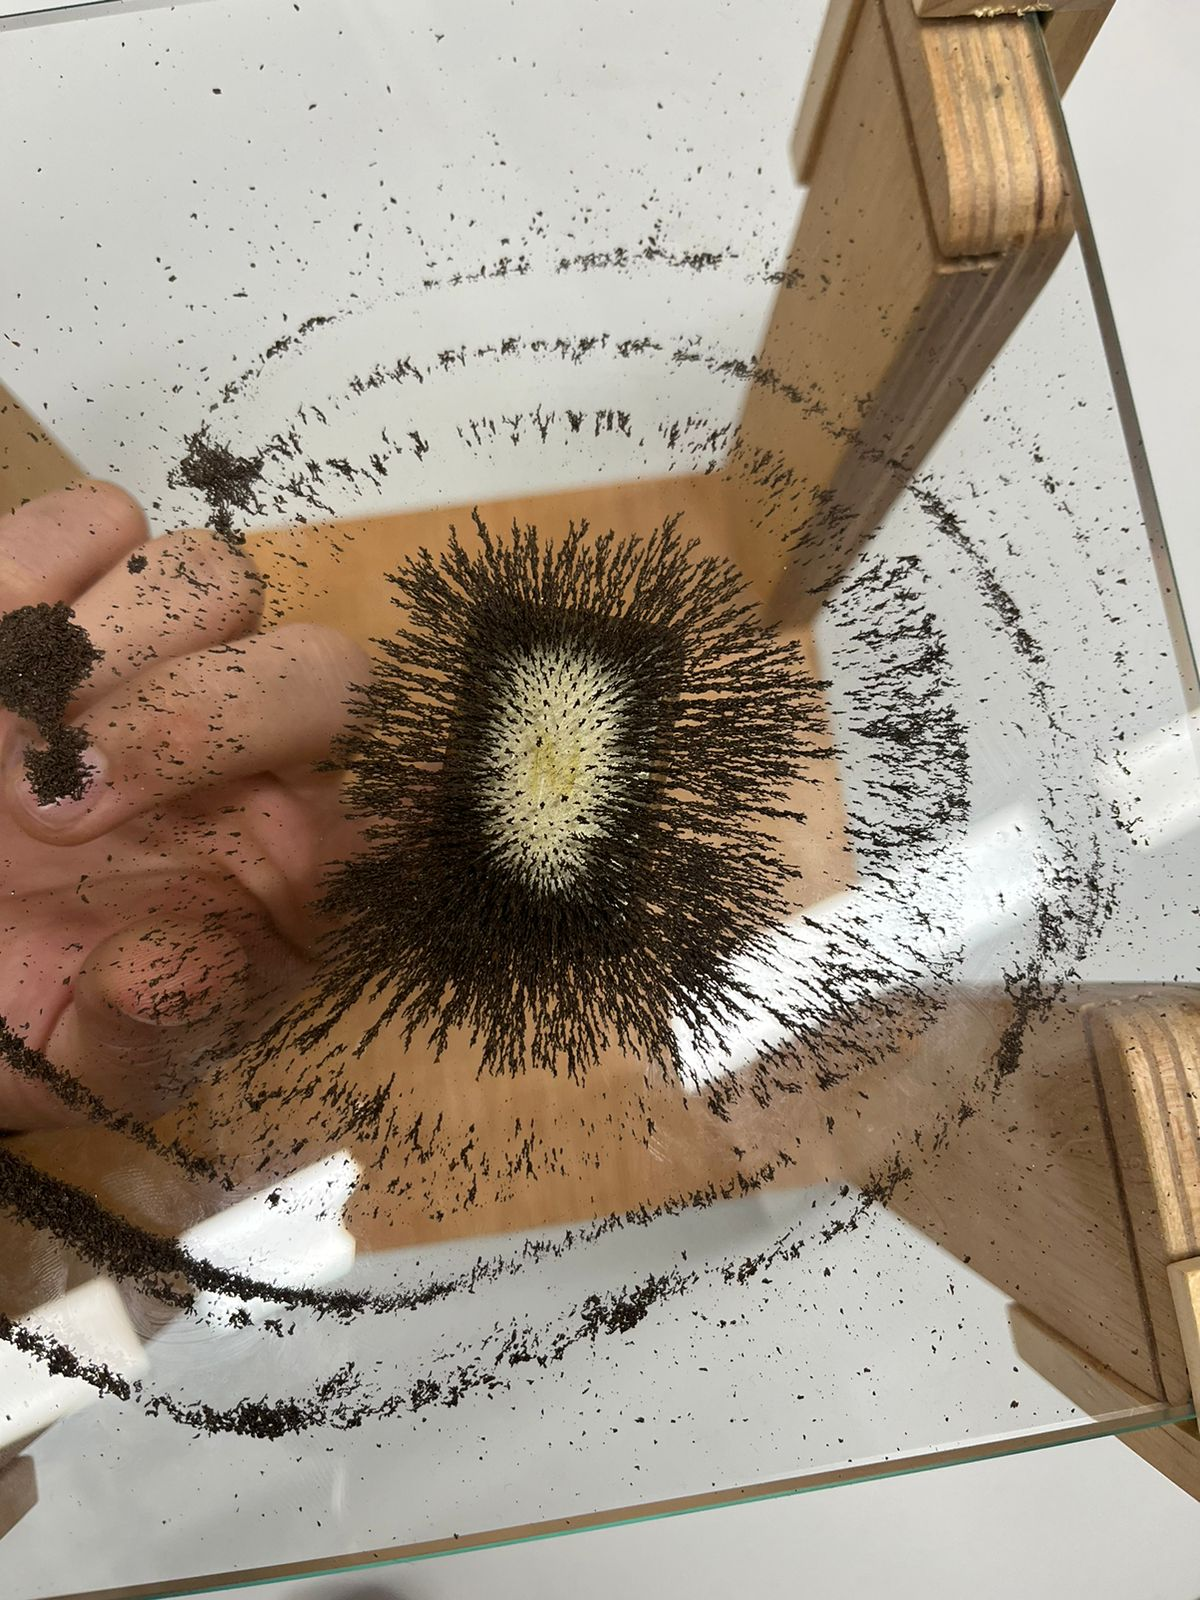
\includegraphics[width=\textwidth]{Figures/1. Content/LimadurasHierro3.jpeg}
    \captionof{figure}{Líneas de campo de limaduras de hierro con imán 1}
    \label{fig: Limadura de Hierro 3}
  \end{minipage}
  \hfill
  \begin{minipage}{0.45\textwidth}
    \centering
    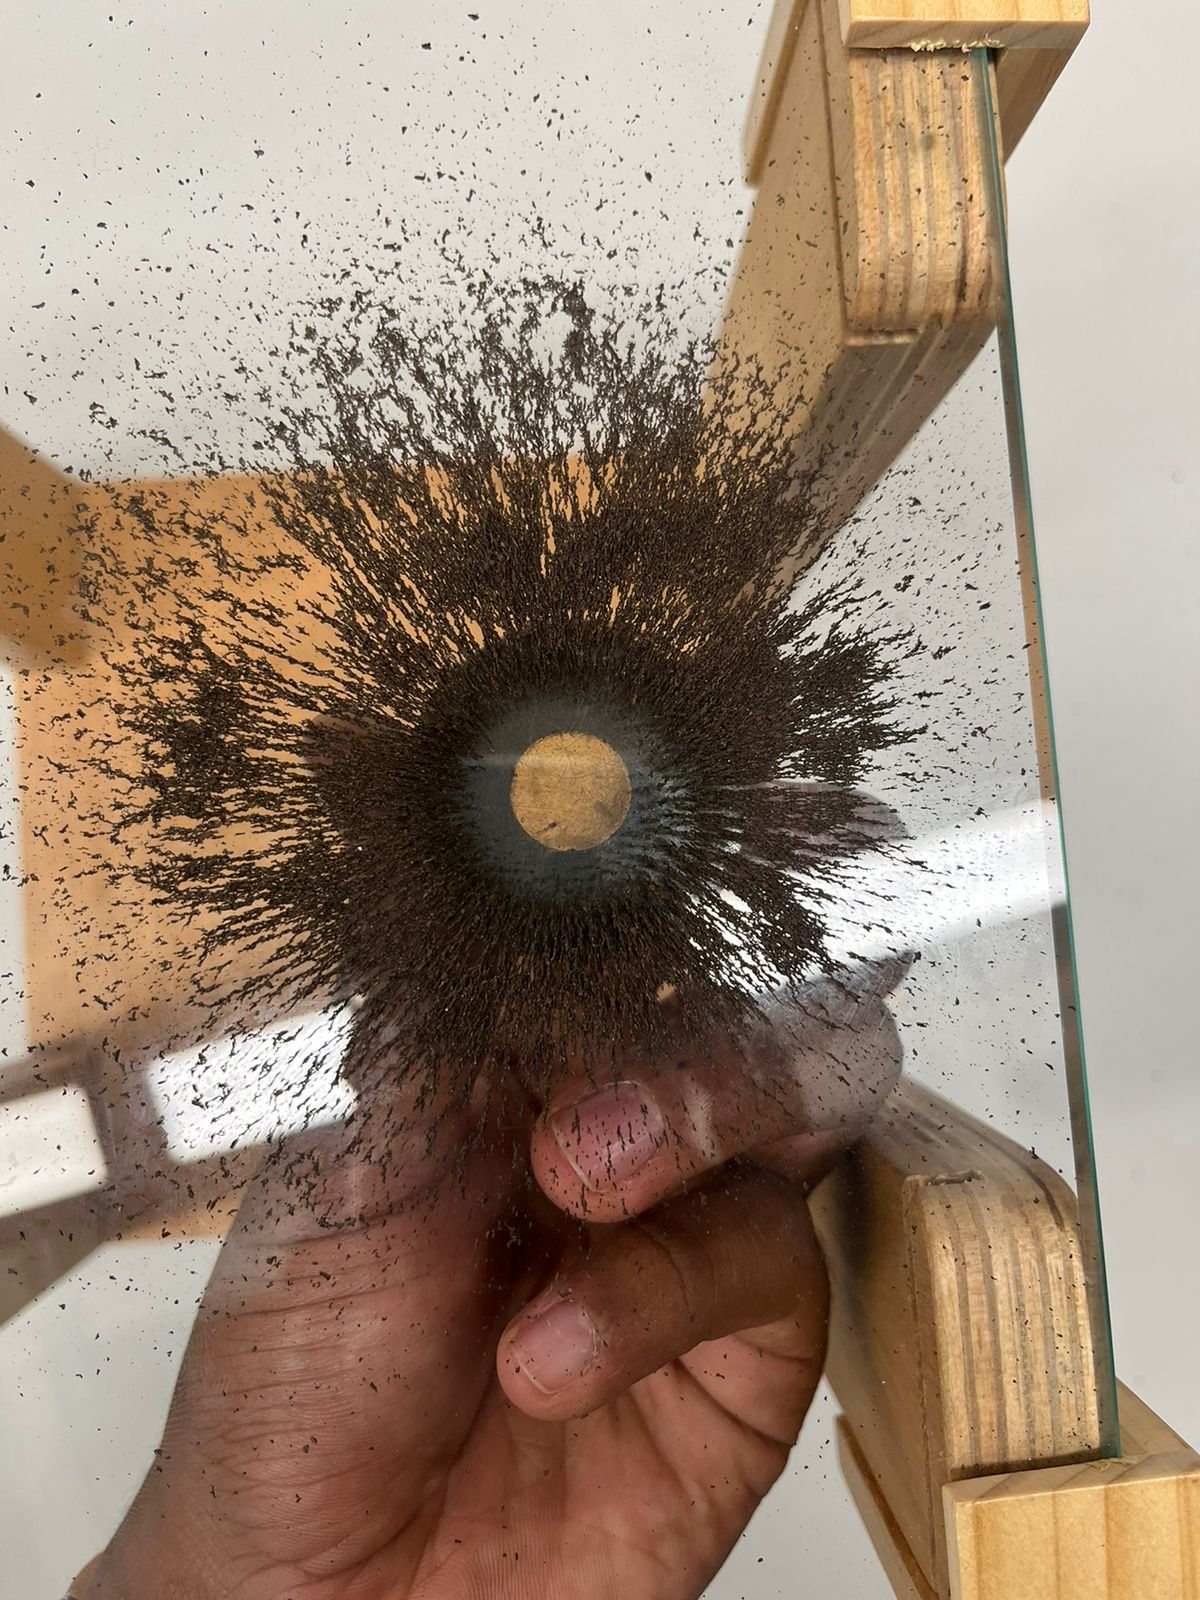
\includegraphics[width=\textwidth]{Figures/1. Content/LimadurasHierro1.jpeg}
    \captionof{figure}{Líneas de campo de limaduras de hierro con imán 2}
    \label{fig: Limadura de Hierro 1}
  \end{minipage}
  \hfill
  \begin{minipage}{0.45\textwidth}
    \centering
    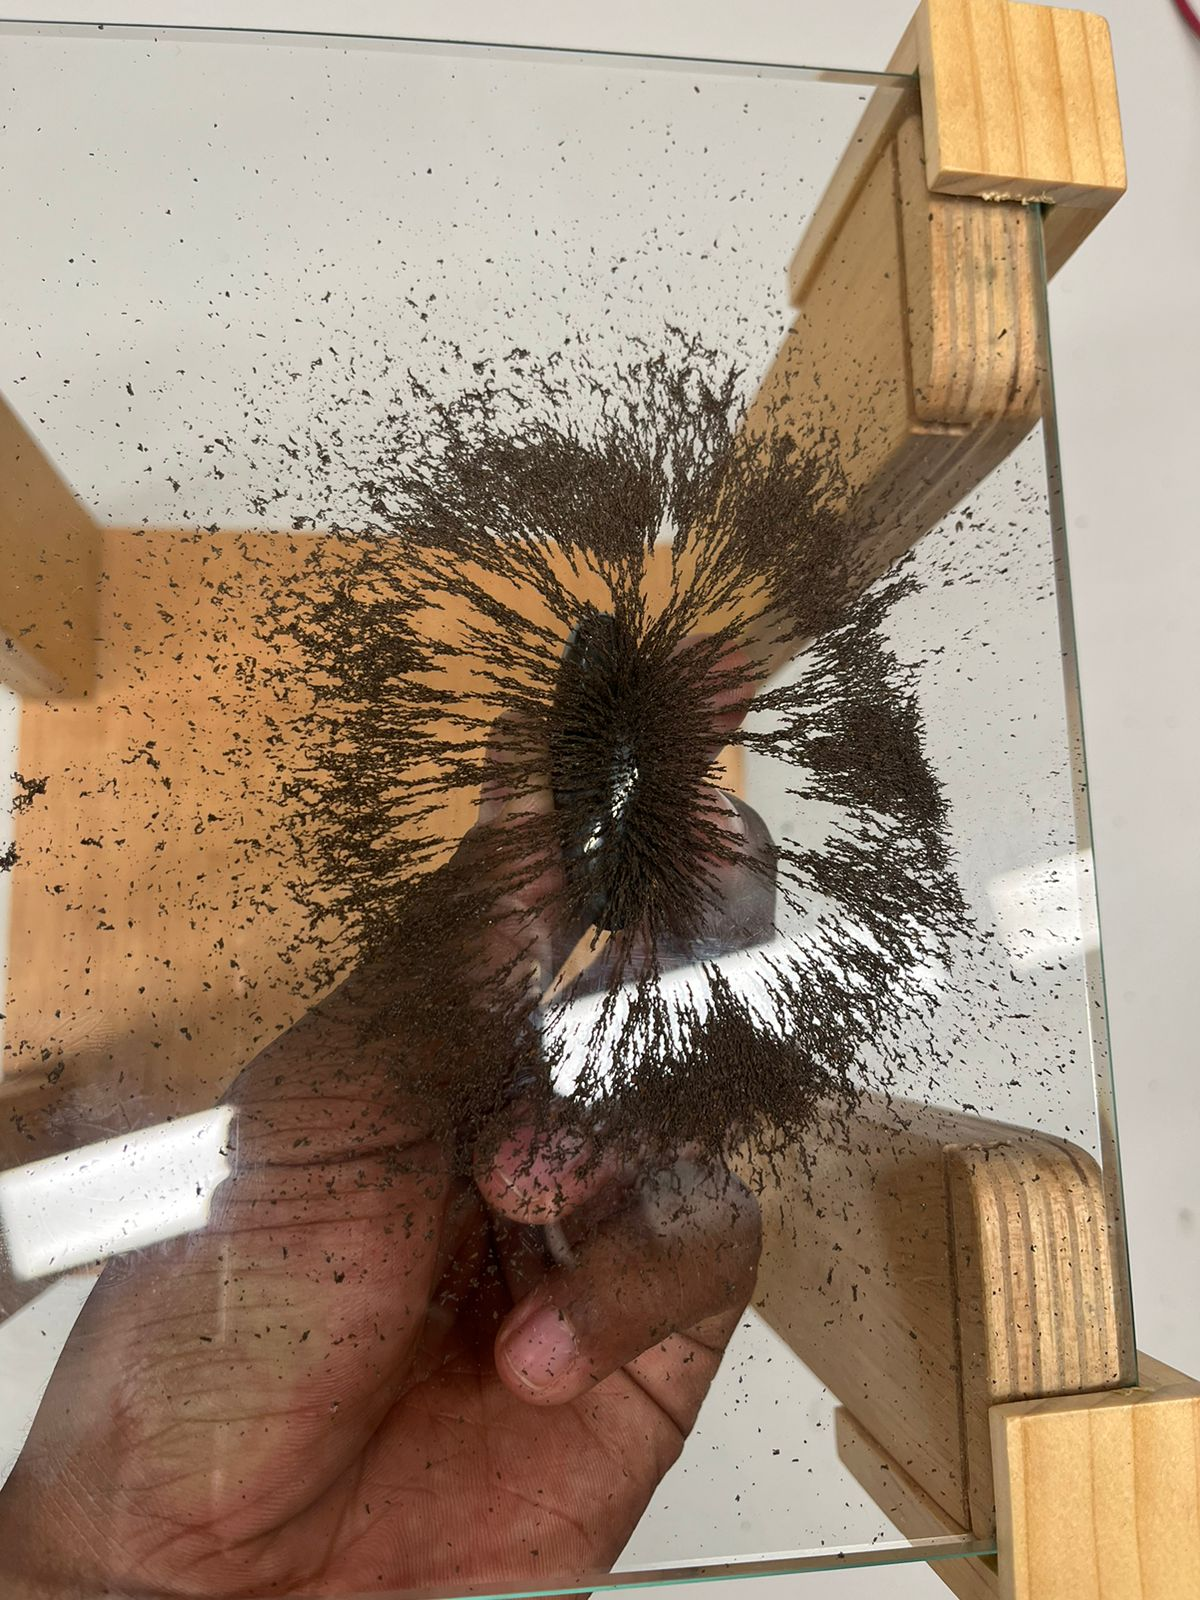
\includegraphics[width=\textwidth]{Figures/1. Content/LimadurasHierro2.jpeg}
    \captionof{figure}{Líneas de campo de limaduras de hierro con imán 3}
    \label{fig: Limadura de Hierro 2}
  \end{minipage}
  \hfill

\end{figure}

\begin{itemize}
  \item \textbf{Imán 1:} Las limaduras se organizaron en un patrón radial alrededor del imán, mostrando un punto central desde donde parece emanar el campo. Esto sugiere un imán con un solo polo dominante visible o un disco magnético con un campo concentrado en el centro.

  \item \textbf{Imán 2:} El patrón formado por las limaduras indica un campo magnético clásico de un dipolo, con líneas que emergen desde un extremo del imán y reingresan en el otro. Esto es típico de un imán de barra, donde las líneas de campo se curvan desde el polo norte hacia el polo sur.

  \item \textbf{Imán 3:} Similar al segundo imán, pero con líneas de campo que se extienden más ampliamente alrededor de los polos, indicando posiblemente un campo más fuerte o un imán de mayor tamaño. Las líneas son más dispersas, lo que sugiere una interacción más fuerte con el entorno circundante.
\end{itemize}

Estas observaciones permiten visualizar y comprender la forma en que el campo magnético interactúa con materiales ferromagnéticos y cómo se manifiesta el flujo magnético en el espacio alrededor de diferentes tipos de imanes.


\subsection{Encontrar los polos de los imanes}
\textbf{Con dos imanes, encuentre los polos norte y sur de cada uno de ellos.
Describa lo que sucede.}

\begin{figure}[H]
  \centering
  \begin{minipage}{0.3\textwidth}
    \centering
    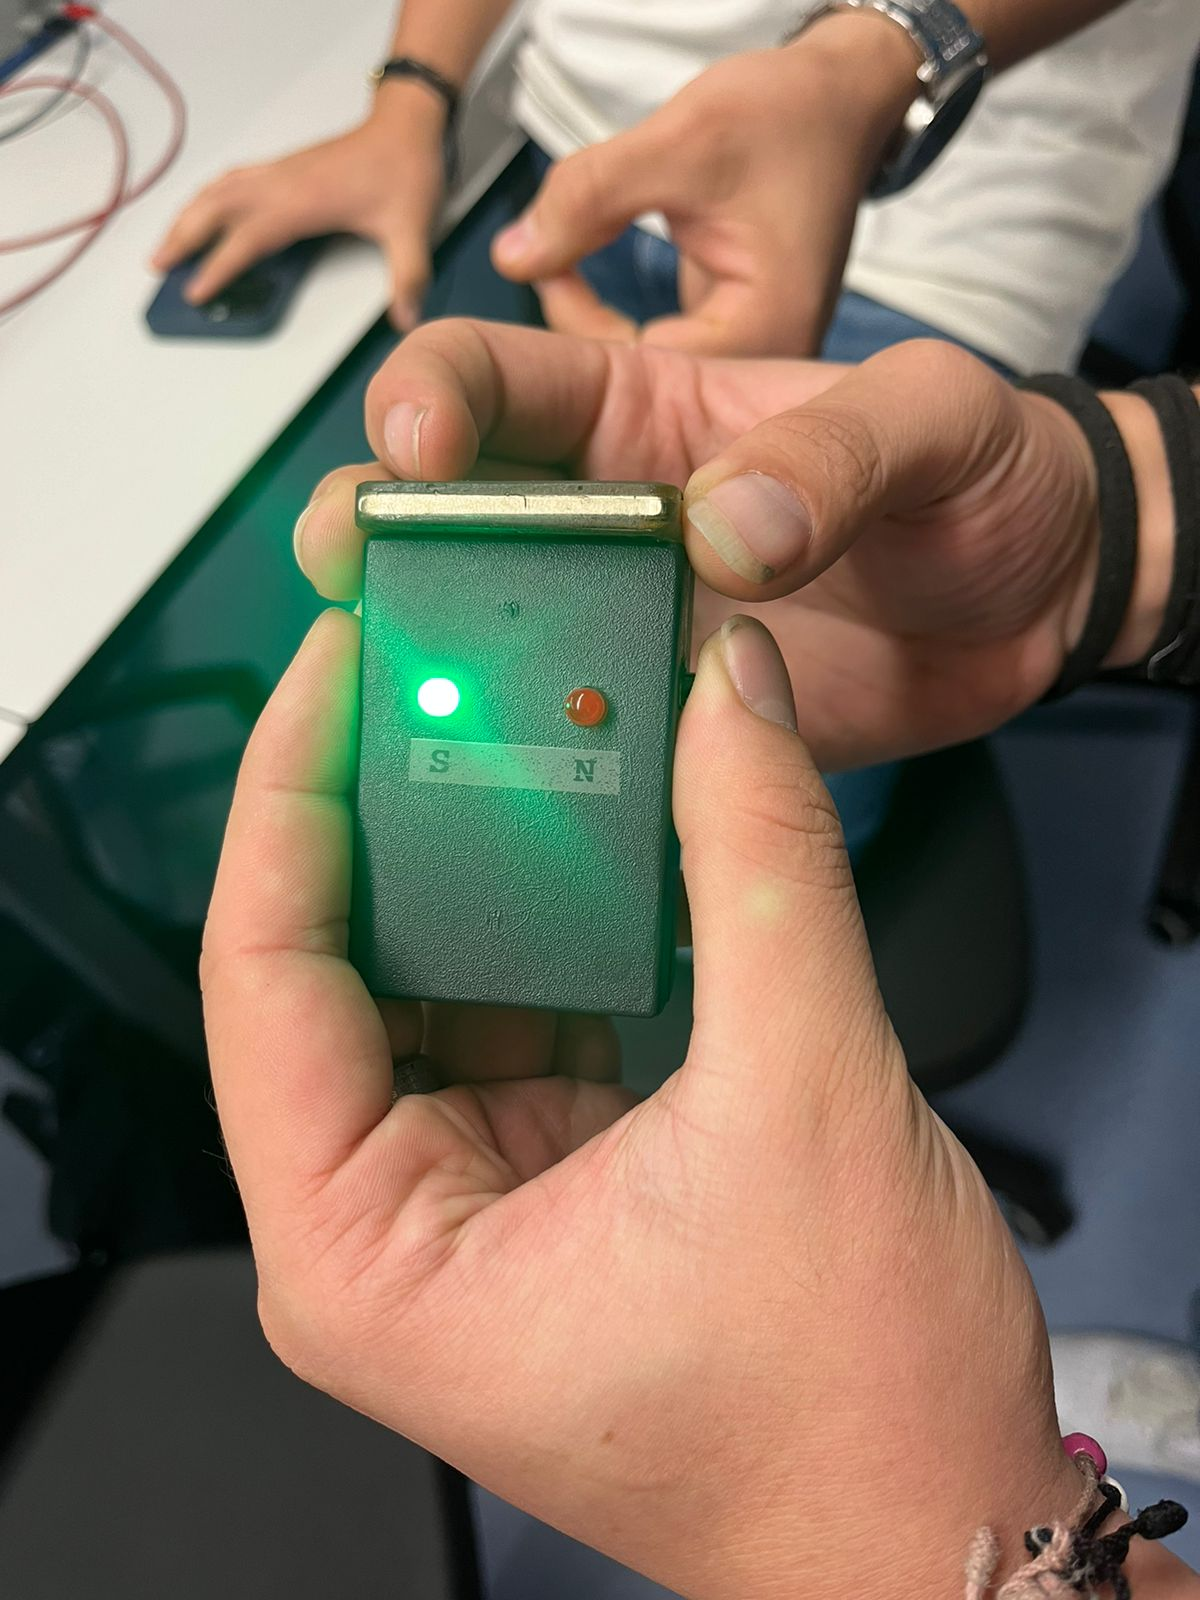
\includegraphics[width=\textwidth]{Figures/1. Content/BuscarPolaridad5.jpeg}
    \captionof{figure}{Polaridad Positiva del Imán 1}
    \label{fig: Polaridad Positiva del Iman 1}
  \end{minipage}
  \hfill
  \begin{minipage}{0.3\textwidth}
    \centering
    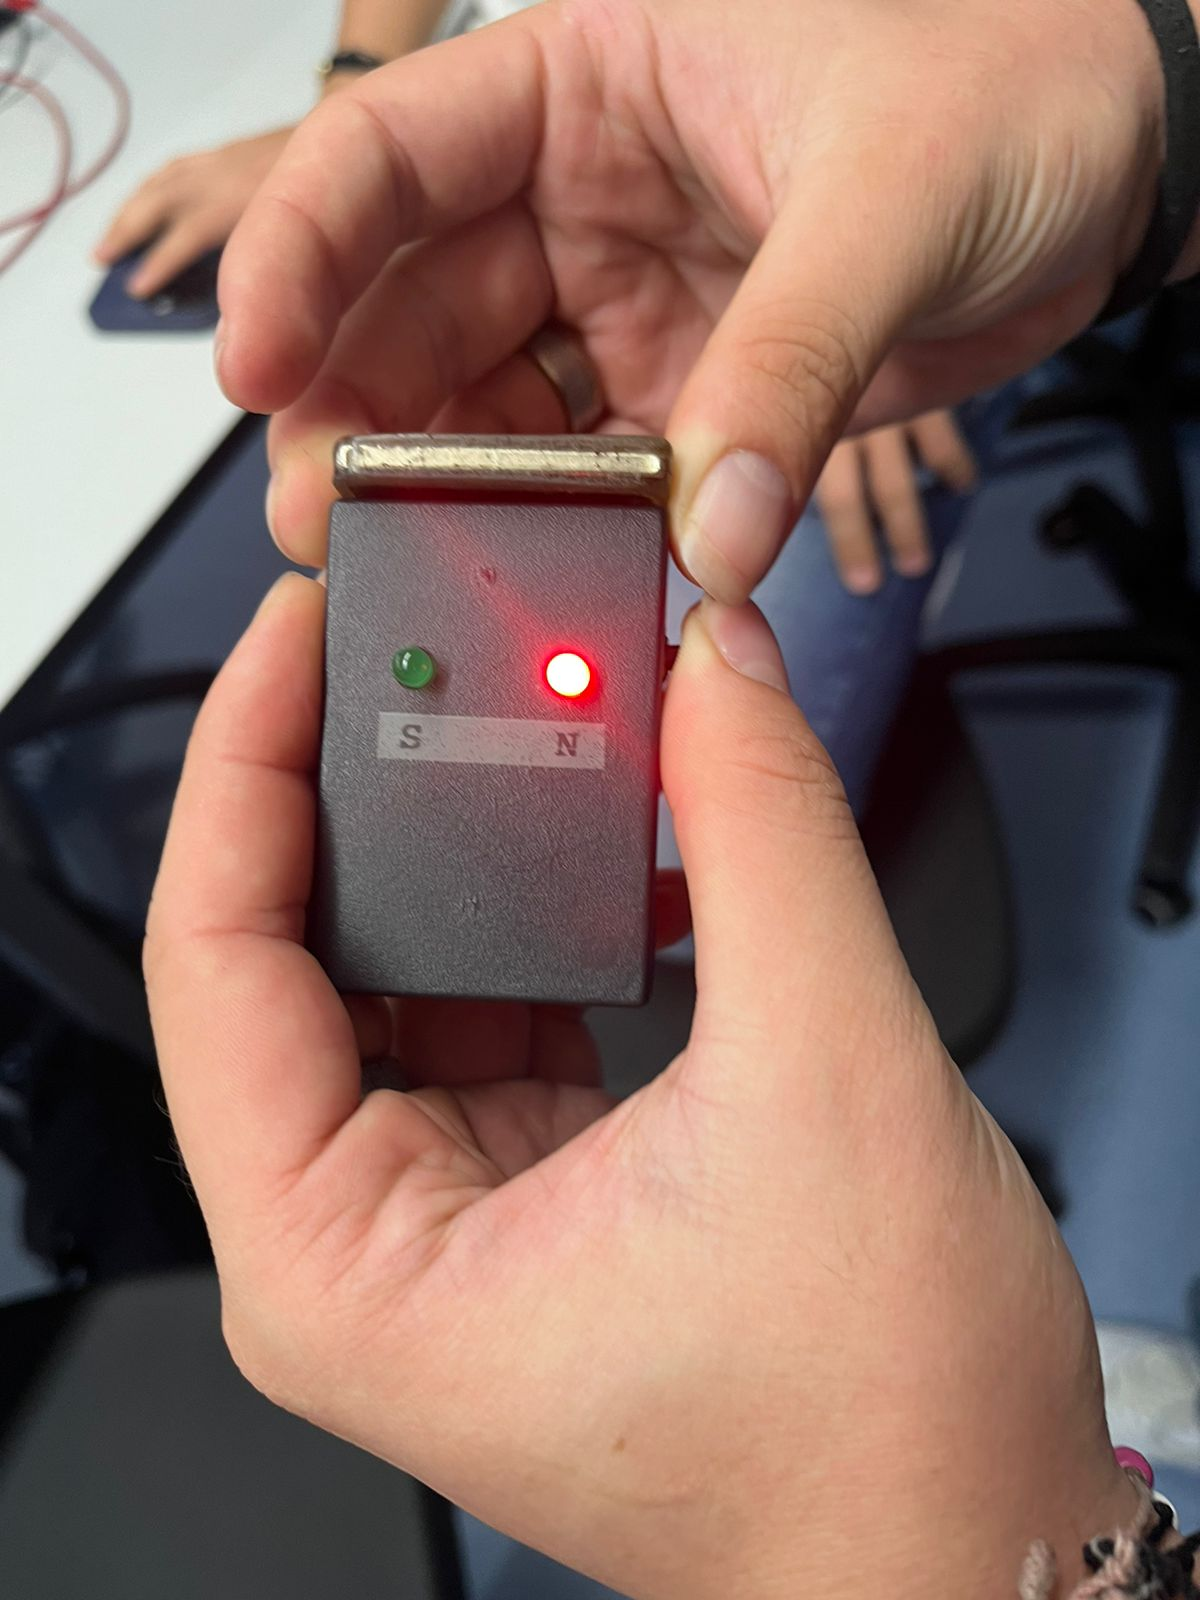
\includegraphics[width=\textwidth]{Figures/1. Content/BuscarPolaridad6.jpeg}
    \captionof{figure}{Polaridad Negativa del Imán 1}
    \label{fig: Polaridad Negativa del Iman 1}
  \end{minipage}
  \hfill
  \begin{minipage}{0.3\textwidth}
    \centering
    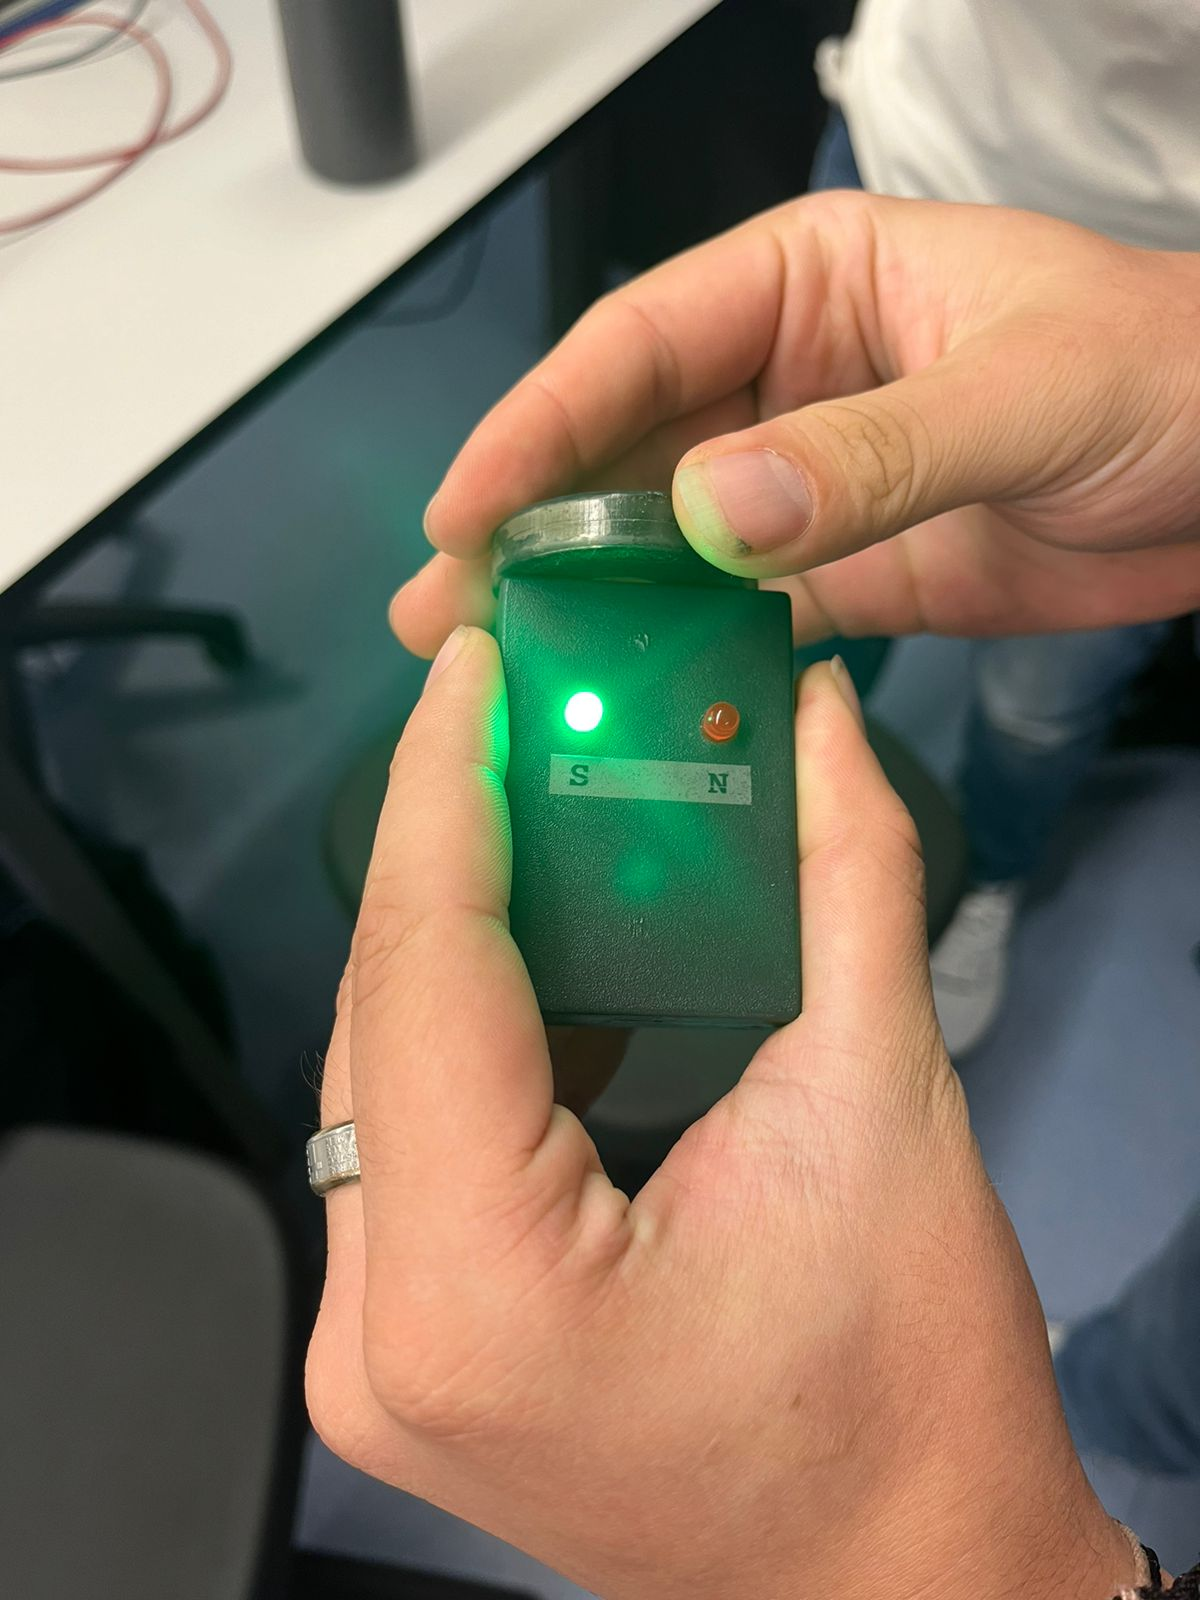
\includegraphics[width=\textwidth]{Figures/1. Content/BuscarPolaridad1.jpeg}
    \captionof{figure}{Polaridad Positiva del Imán 2}
    \label{fig: Polaridad Positiva del Iman 2}
  \end{minipage}
  \hfill
  \begin{minipage}{0.3\textwidth}
    \centering
    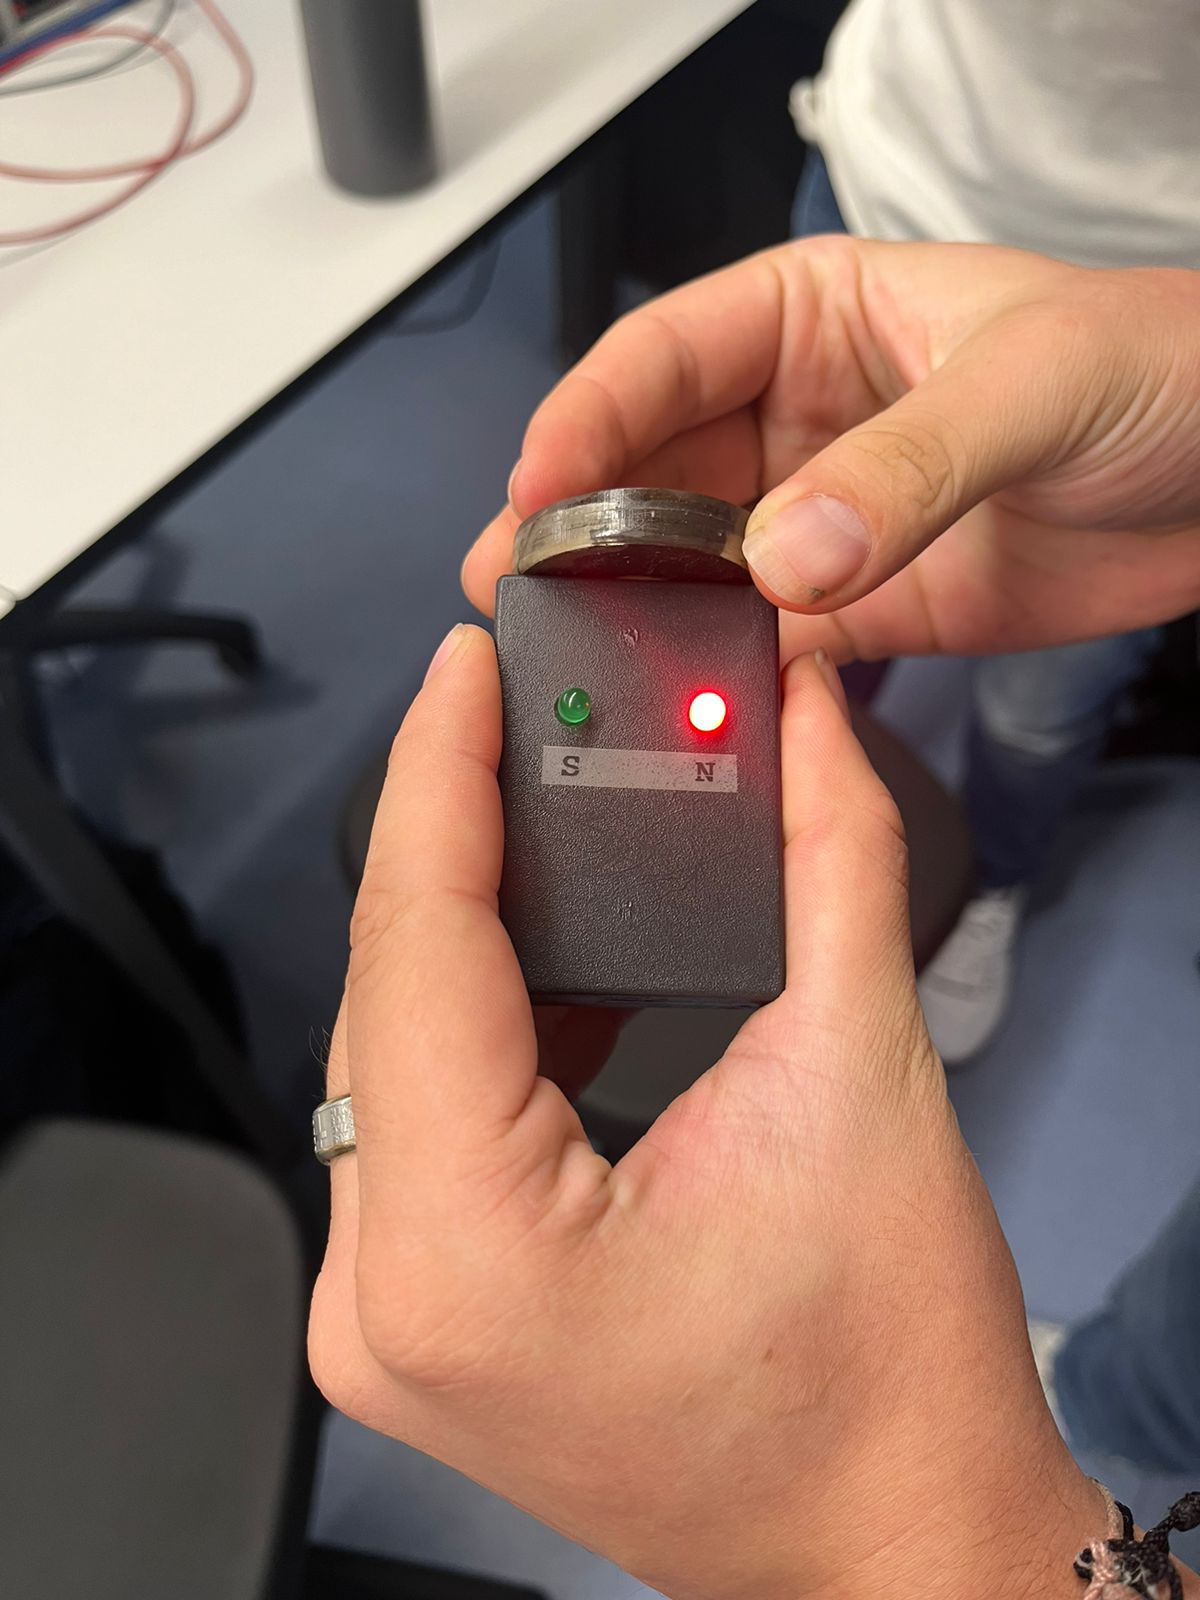
\includegraphics[width=\textwidth]{Figures/1. Content/BuscarPolaridad2.jpeg}
    \captionof{figure}{Polaridad Negativa del Imán 2}
    \label{fig: Polaridad Negativa del Iman 2}
  \end{minipage}
  \hfill
  \begin{minipage}{0.3\textwidth}
    \centering
    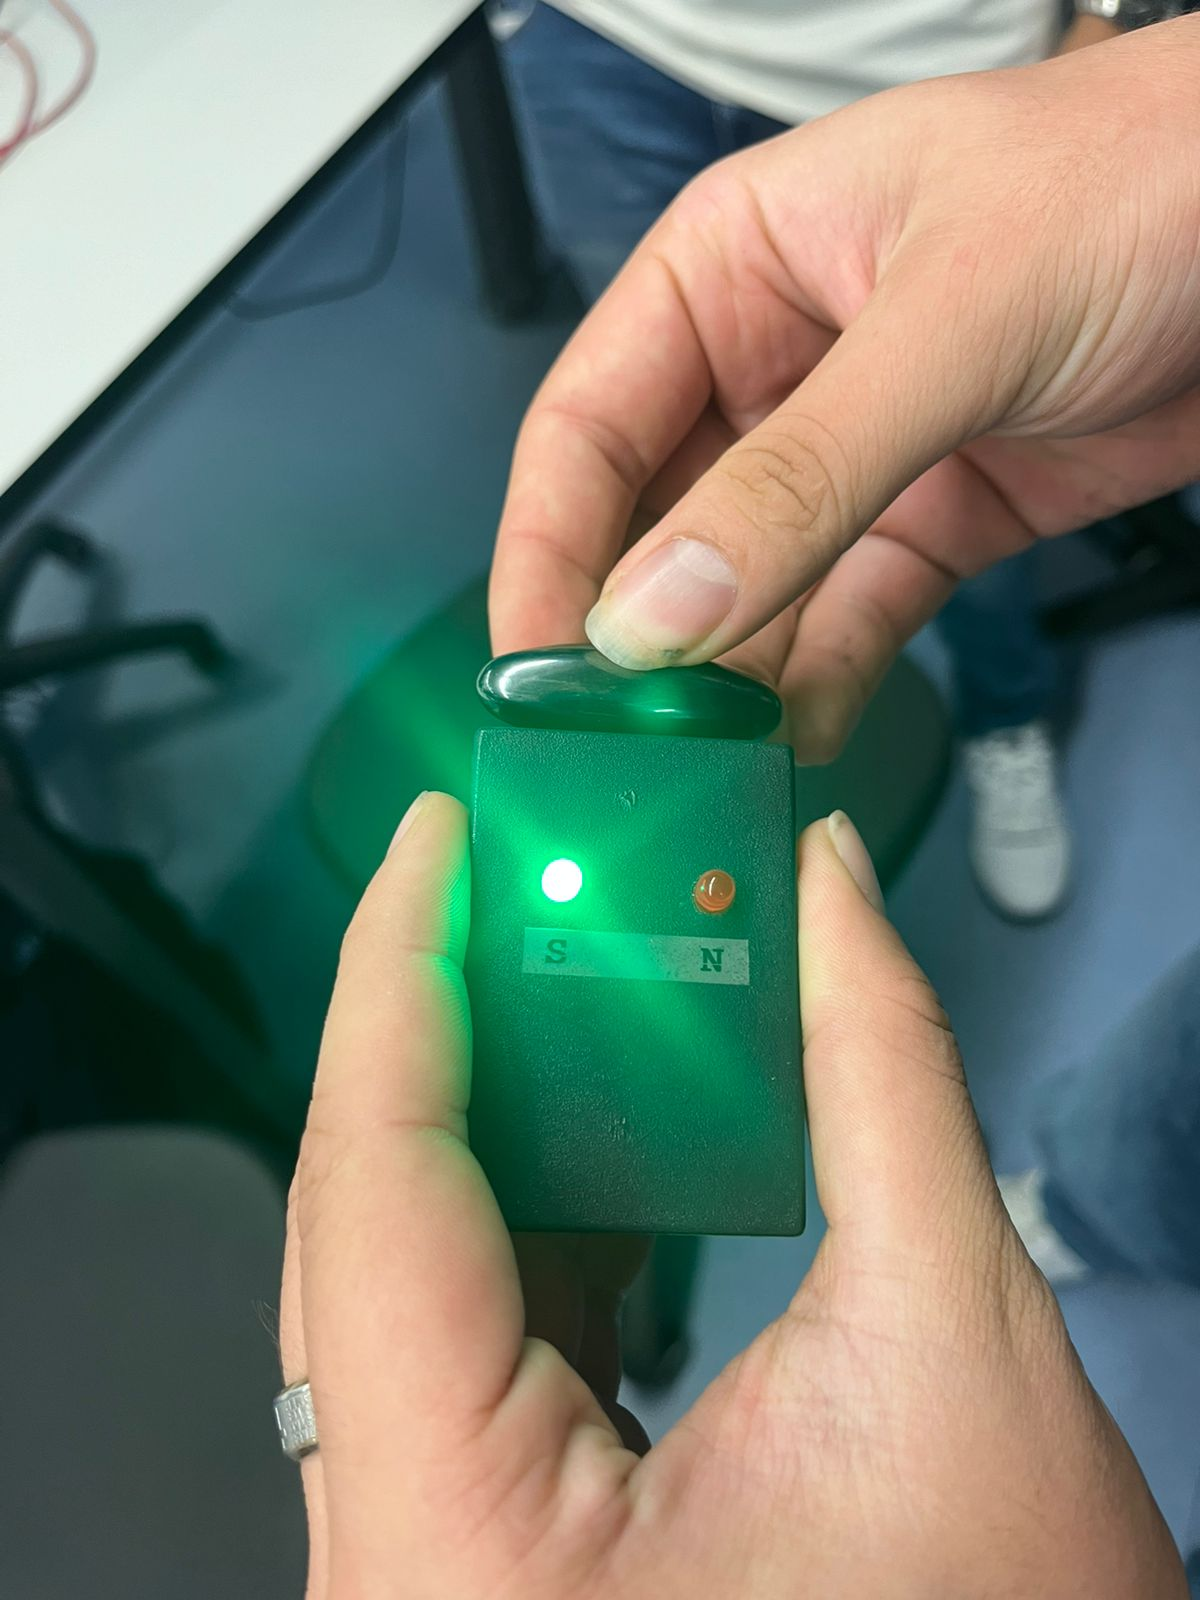
\includegraphics[width=\textwidth]{Figures/1. Content/BuscarPolaridad3.jpeg}
    \captionof{figure}{Polaridad Positiva del Imán 3}
    \label{fig: Polaridad Positiva del Iman 3}
  \end{minipage}
  \hfill
  \begin{minipage}{0.3\textwidth}
    \centering
    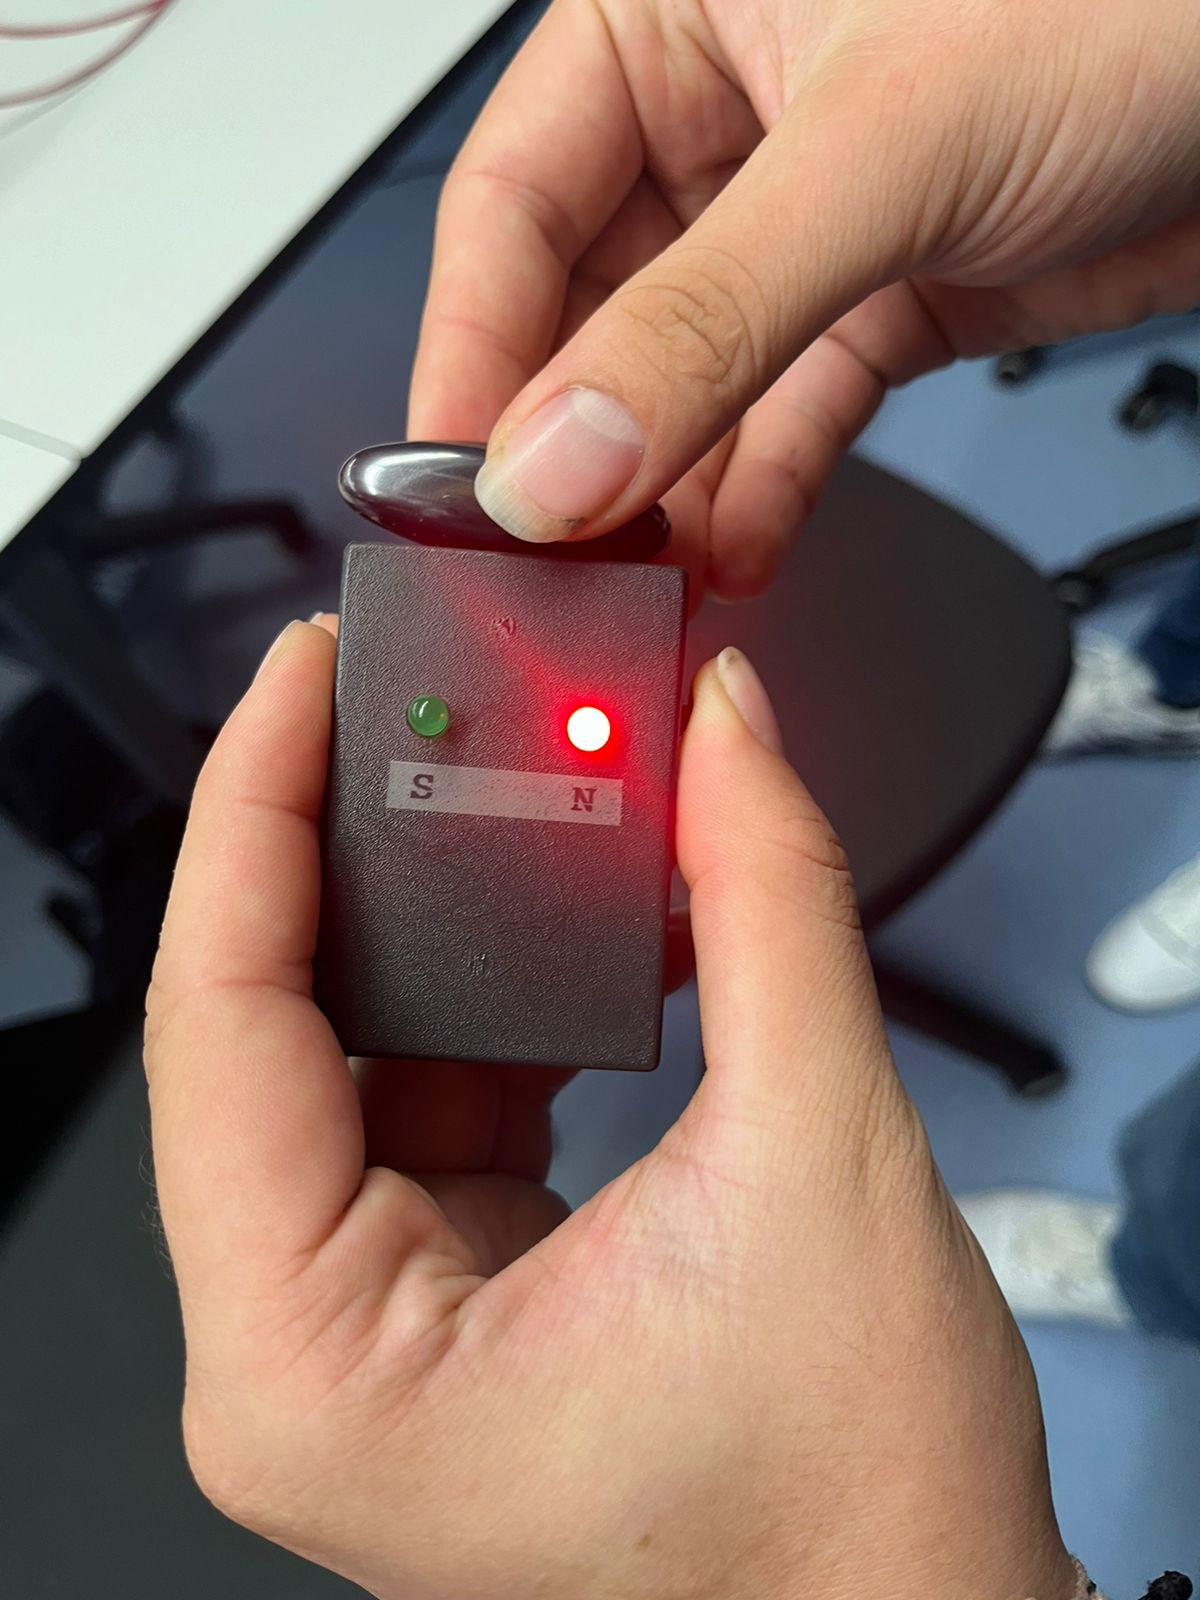
\includegraphics[width=\textwidth]{Figures/1. Content/BuscarPolaridad4.jpeg}
    \captionof{figure}{Polaridad Negativa del Imán 3}
    \label{fig: Polaridad Negativa del Iman 3}
  \end{minipage}
  \hfill
\end{figure}

Para identificar los polos de los imanes, se utilizó un dispositivo detector de polaridad que indica mediante luces LED el tipo de polo que se está examinando: verde para el polo norte y rojo para el polo sur. Al aproximarse los imanes uno hacia el otro, observamos las siguientes reacciones:

\begin{itemize}
    \item Cuando los polos opuestos de dos imanes se acercan (norte con sur), las luces indicadoras muestran colores diferentes en cada imán (uno verde y el otro rojo), lo cual indica una atracción. Este fenómeno es consistente con la ley de magnetismo que dicta que polos opuestos se atraen.
    \item Al enfrentar los mismos polos (norte con norte o sur con sur), las luces muestran el mismo color en ambos imanes, indicando que estamos frente a polos iguales. En esta configuración, se observa una repulsión clara entre los imanes, donde cada uno intenta alejarse del otro, validando la ley que polos iguales se repelen.
\end{itemize}

Estas observaciones no solo confirmaron la funcionalidad del detector de polaridad, sino que también proporcionaron una visualización directa e interactiva de las interacciones fundamentales entre los campos magnéticos de los imanes.


\subsection{Comprobación de Interacciones Magnéticas}
\textbf{Para dos imanes compruebe que polos magnéticos del mismo tipo se repelen y polos magnéticos de distinto tipo se atraen. Para las siguientes situaciones, observe las posiciones en donde la atracción es máxima y las posiciones en donde la repulsión es máxima. Igualmente, se trata de visualizar el campo magnético con limaduras de hierro.}

En esta serie de experimentos, utilizamos dos imanes y limaduras de hierro para visualizar las líneas de campo magnético y verificar las interacciones entre diferentes configuraciones de polos:

\begin{enumerate}
    \item \textbf{Un imán solo:} Con un solo imán bajo una hoja de vidrio espolvoreada con limaduras de hierro, observamos cómo las limaduras se alinean a lo largo de las líneas del campo magnético, emanando del polo norte hacia el polo sur del imán, creando un patrón conocido de campo magnético.

    \item \textbf{Dos imanes con polos idénticos enfrentados:} Al enfrentar los polos norte con norte o sur con sur, las limaduras de hierro revelan un campo donde las líneas intentan alejarse una de la otra, indicando repulsión. Esta configuración mostró un claro espacio vacío entre los polos enfrentados donde las limaduras se repelían, evidenciando la máxima repulsión.

    \item \textbf{Dos imanes con polos opuestos enfrentados:} Contrariamente, al alinear los polos opuestos (norte con sur), las limaduras formaron un puente directo entre los dos imanes, indicando una fuerte atracción. Las limaduras se alinearon densamente entre los dos polos, mostrando la zona de máxima atracción donde las líneas de campo se unen directamente.
\end{enumerate}

Estos experimentos no solo demostraron visualmente las fuerzas fundamentales de atracción y repulsión magnética, sino que también permitieron observar cómo el campo magnético se distorsiona y adapta según la configuración de los imanes.

\subsection{Medición del Campo Magnético y Determinación de la Fuerza Magnética}
Medimos el campo magnético a una distancia constante utilizando un teslámetro para tres diferentes imanes: un imán rectangular, un imán circular, y un imán en forma de Elipsoide. Las mediciones se realizaron a distancias incrementales desde la superficie del imán hasta 8 mm. Los resultados son los siguientes:

\begin{itemize}
    \item \textbf{Imán 1 (Rectangular)}: Este imán mostró los valores más altos de campo magnético, empezando en 33.1 mT en la superficie y disminuyendo hasta 4.6 mT a una distancia de 8 mm.
    \item \textbf{Imán 2 (Circular)}: Este imán comenzó con un campo de 11.6 mT en la superficie, reduciéndose a 1.6 mT a 8 mm.
    \item \textbf{Imán 3 (Elipsoide)}: El campo magnético comenzó en 14.7 mT y bajó a 1.9 mT a 8 mm de distancia.
\end{itemize}

Los gráficos de la variación del campo magnético en función de la distancia muestran que el \textbf{Imán 1 (Rectangular)} tiene la mayor fuerza magnética en todas las distancias medidas, seguido por el \textbf{Imán 3 (Elipsoide)} y luego el \textbf{Imán 2 (Circular)}. Esto se refleja también en los cálculos de potencia, donde el imán rectangular domina significativamente en términos de influencia magnética a corta distancia.

Estos resultados sugieren que la geometría del imán juega un papel crucial en su capacidad para mantener un campo magnético a mayores distancias, con el imán rectangular mostrando la mayor eficacia en retener su fuerza magnética comparado con las formas circular y esférica.

\subsection{Tabla de cada imán}
\textbf{De acuerdo con la geometría del teslámetro construya la siguiente tabla, midiendo
el campo magnético de tres imanes diferentes a diferentes distancias.}


\section{Procedimiento Experimental y Resultados: Montaje 2 Resistencias en Paralelo}

\subsection{Conecte el circuito de la Figura 3}
\textbf{Conecte el circuito de la siguiente figura:}
\begin{figure}[H]
    \centering
    \begin{subfigure}[b]{\textwidth}
        \centering
        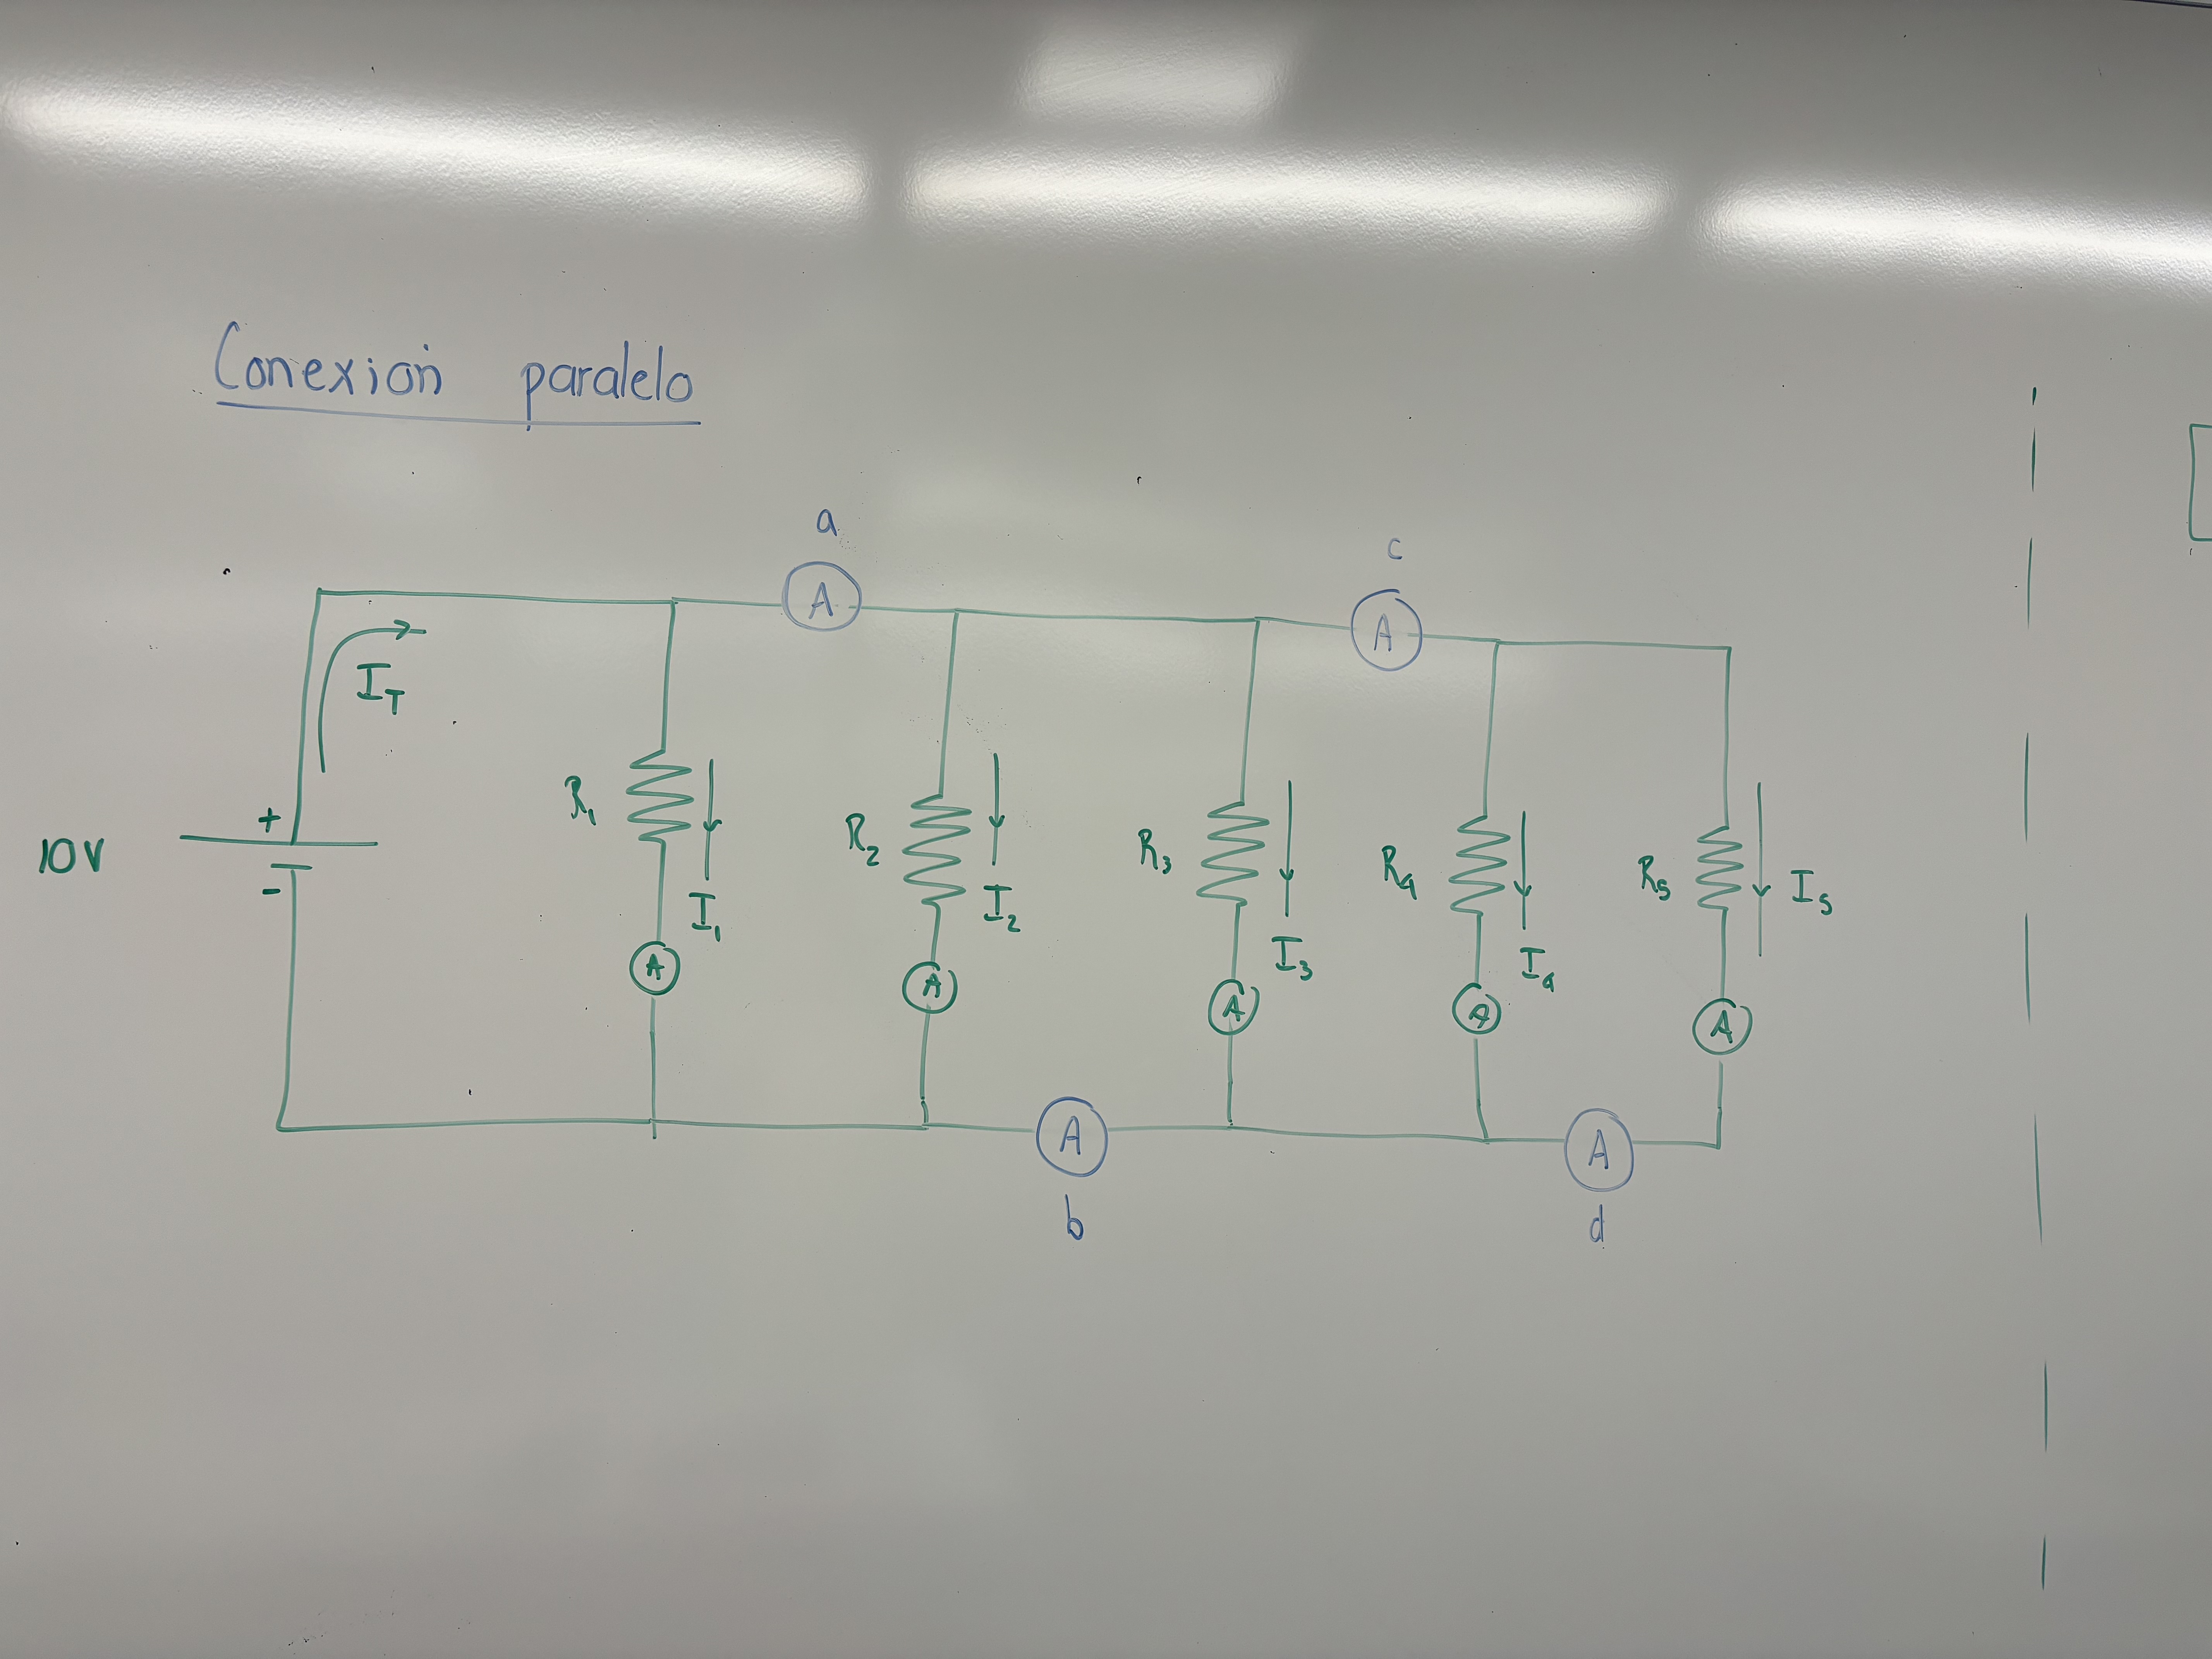
\includegraphics[width=0.8\textwidth]{Figures/1. Content/ConexionParalelo.jpg}
        \caption{Conexión en Paralelo}
        \label{fig: Conexion Paralelo}
    \end{subfigure}
    \hfill
\end{figure}

\subsection{Corriente en cada resistor}
\textbf{Con el amperímetro mida y reporte la corriente entregada por la fuente y a través de cada resistor:}

La corriente medida a través de cada resistor se presenta en la siguiente tabla:

\begin{table}[h]
\centering
\begin{tabular}{|c|c|c|c|c|c|}
\hline
\(I (A)\) & \(I_1 (A)\) & \(I_2 (A)\) & \(I_3 (A)\) & \(I_4 (A)\) & \(I_5 (A)\) \\ \hline
$0.471$     & $0.205$       & $0.052$       & $0.025$       & $0.116$       & $0.076$       \\ \hline
\end{tabular}
\caption{Corrientes medidas en cada punto del circuito.}
\label{tab:current_measurements}
\end{table}

Esta tabla muestra de manera organizada la distribución de la corriente a través de cada resistor, además de la corriente total medida directamente de la fuente.

\subsection{Cálculo de la Suma de Corrientes}
\textbf{Calcule \(I_1 + I_2 + I_3 + I_4 + I_5 = \_\_\_\_\_ \)}
La suma de las corrientes a través de cada resistor se calculó como:
\[
I_1 + I_2 + I_3 + I_4 + I_5 = 0.205 + 0.052 + 0.025 + 0.116 + 0.076 = 0.474 \, \text{A}
\]
Esta suma es muy cercana al valor de corriente total medido, \(0.471 \, \text{A}\), y está dentro de lo esperado considerando posibles errores de medición.

\subsection{Comparación de la Corriente Total}
\textbf{¿Cómo es la corriente entregada por la fuente comparada con el resultado de 2.2? Explique.}
La corriente total entregada por la fuente, \(0.471 \, \text{A}\), es casi idéntica a la suma de las corrientes a través de cada componente del circuito, \(0.474 \, \text{A}\). Esta pequeña discrepancia entre los valores puede atribuirse a errores menores en la medición y la precisión del amperímetro. Este resultado confirma la ley de conservación de la carga, que postula que la corriente total en un circuito cerrado debe ser constante y equivalente a la suma de las corrientes que fluyen a través de cada componente del circuito.

\subsection{Corriente nodo $a$}
\textbf{¿Qué valor tiene la corriente que sale del nodo $a$?} \underline{$0.219$}


\subsection{Corriente nodo $b$}
\textbf{¿Qué valor tiene la corriente que sale del nodo $a$?} \underline{$0.218$}


\subsection{Corriente nodo $c$}
\textbf{¿Qué valor tiene la corriente que sale del nodo $a$?} \underline{$0.193$}


\subsection{Corriente nodo $d$}
\textbf{¿Qué valor tiene la corriente que sale del nodo $a$?} \underline{$0.115$}

\subsection{Voltaje en cada resistor}
\textbf{Mida y reporte el voltaje en cada resistor:}

El voltaje medido a través de cada resistor se presenta en la siguiente tabla:

\begin{table}[h]
\centering
\begin{tabular}{|c|c|c|c|c|c|}
\hline
\(V_{Fuente} (V)\) & \(V_1 (V)\) & \(V_2 (V)\) & \(V_3 (V)\) & \(V_4 (V)\) & \(V_5 (V)\) \\ \hline
$10.3$     & $10.42$       & $10.39$       & $10.48$       & $10.46$       & $10.45$       \\ \hline
\end{tabular}
\caption{Voltajes medidas en cada punto del circuito.}
\label{tab:volt_measurements}
\end{table}

\subsection{Voltaje en Cada Resistor Comparado con la Fuente}
\textbf{¿Cómo es el voltaje en cada resistor comparado con el voltaje entregado por la fuente? Explique.}
Los voltajes medidos en cada resistor (aproximadamente 10.4 V para cada uno) son sorprendentemente similares y ligeramente superiores al voltaje teórico de la fuente (10 V) y al experimental medido directamente (10.3 V). Esto puede atribuirse a pequeños errores de medición o variaciones en la carga real en el momento de las mediciones. El hecho de que todos los resistores muestren voltajes similares también indica que la caída de tensión a lo largo del circuito es uniforme, lo que es típico en circuitos en serie donde la misma corriente fluye a través de cada componente.

\section{Interacción de las Resistencias Internas de los Equipos de Medida}
\textbf{Sabiendo que tanto el voltímetro como el amperímetro son equipos que poseen resistencias internas, ¿cuál es la razón para que estas no interactúen con la medida?}
Los amperímetros están diseñados para tener una resistencia interna muy baja para minimizar su impacto en el circuito cuando se conectan en serie, lo cual podría alterar la corriente que se está midiendo. Los voltímetros, por otro lado, tienen una resistencia interna muy alta para evitar la extracción de corriente significativa del punto de medición, lo que podría afectar la tensión que se está midiendo.

\section{Importancia de Resistencias y Condensadores Equivalentes}
\textbf{¿Qué importancia tiene poder tener resistencias o condensadores equivalentes en un circuito?}
Las resistencias y condensadores equivalentes permiten simplificar el análisis y diseño de circuitos complejos. Al reemplazar un grupo de componentes en serie o paralelo por un único componente equivalente, se puede calcular más fácilmente el comportamiento general del circuito, especialmente en los casos de análisis de respuesta en frecuencia y carga dinámica.

\section{Conexión de Amperímetros en Serie}
\textbf{¿Por qué los amperímetros deben conectarse en serie en el circuito?}
Los amperímetros deben conectarse en serie para poder medir la totalidad de la corriente que fluye a través del circuito. Si se conectaran de otra manera, como en paralelo, podrían cortocircuitar el circuito en el punto de medición o no medir correctamente la corriente que pasa por otros componentes del circuito.

\section{Procedimiento Experimental y Resultados: Montaje 3 Simulaciones en TinkerCad}

\subsection{Conexiones en Serie}
\begin{figure}[H]
    \centering
    \begin{minipage}{0.45\textwidth}
      \centering
      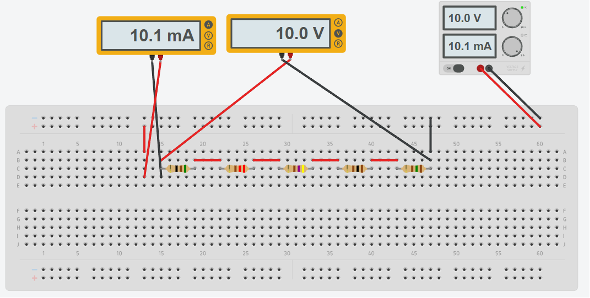
\includegraphics[width=\textwidth]{Figures/1. Content/simulation/serie.png}
      \captionof{figure}{Simulación Conexión en Serie}
      \label{fig: Simulacion Conexion Serie}
    \end{minipage}
    \hfill
    \begin{minipage}{0.45\textwidth}
      \centering
      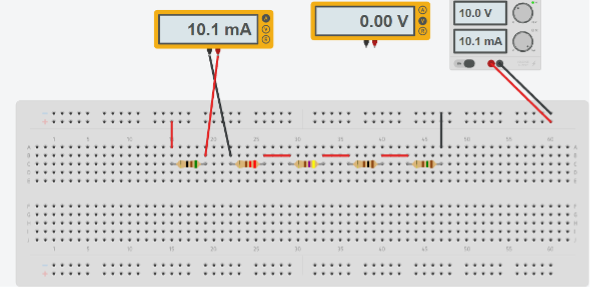
\includegraphics[width=\textwidth]{Figures/1. Content/simulation/serieA1.png}
      \captionof{figure}{Simulación Conexión en Serie $I_{R_1-R_2}$}
      \label{fig: Simulacion Conexion Serie A1}
    \end{minipage}
    \hfill
    \begin{minipage}{0.45\textwidth}
      \centering
      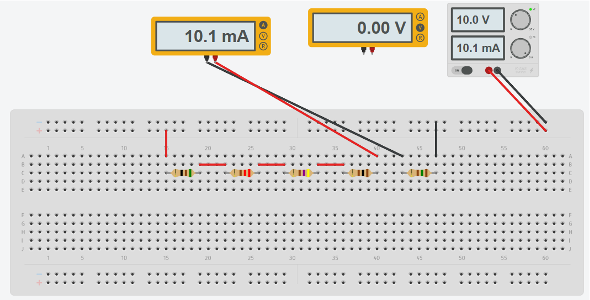
\includegraphics[width=\textwidth]{Figures/1. Content/simulation/serieA2.png}
      \captionof{figure}{Simulación Conexión en Serie $I_{R_4-R_5}$}
      \label{fig: Simulacion Conexion Serie A2}
    \end{minipage}
    \hfill
    \begin{minipage}{0.45\textwidth}
      \centering
      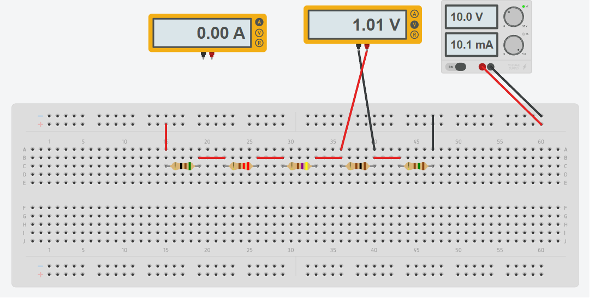
\includegraphics[width=\textwidth]{Figures/1. Content/simulation/serieV1.png}
      \captionof{figure}{Simulación Conexión en Serie $V_{R_4}$}
      \label{fig: Simulacion Conexion Serie V1}
    \end{minipage}
    \hfill
    \begin{minipage}{0.45\textwidth}
      \centering
      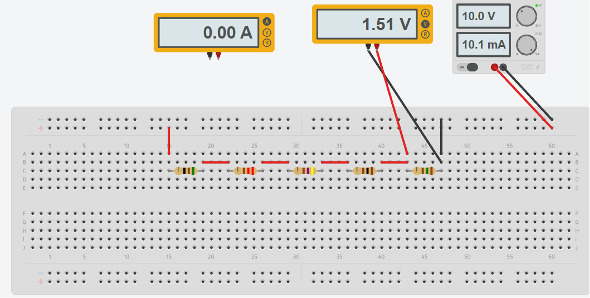
\includegraphics[width=\textwidth]{Figures/1. Content/simulation/serieV2.png}
      \captionof{figure}{Simulación Conexión en Serie $V_{R_5}$}
      \label{fig: Simulacion Conexion Serie V2}
    \end{minipage}
\end{figure}

\subsection{Conexiones en Paralelo}
\begin{figure}[H]
    \centering
    \begin{minipage}{0.45\textwidth}
      \centering
      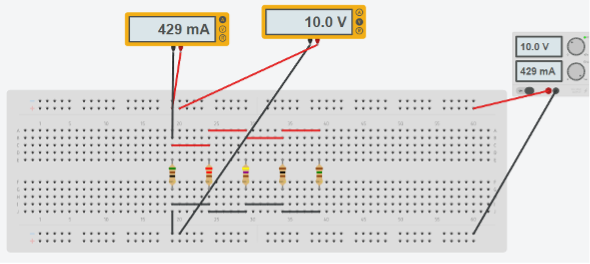
\includegraphics[width=\textwidth]{Figures/1. Content/simulation/paralelo.png}
      \captionof{figure}{Simulación Conexión en Paralelo}
      \label{fig: Simulacion Conexion Paralelo}
    \end{minipage}
    \hfill
    \begin{minipage}{0.45\textwidth}
      \centering
      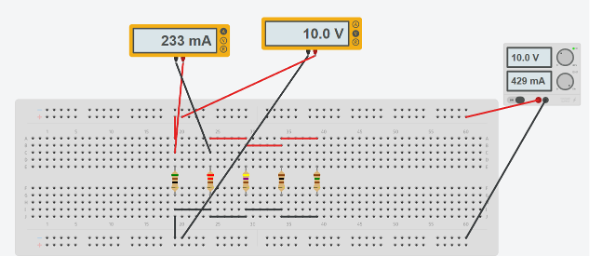
\includegraphics[width=\textwidth]{Figures/1. Content/simulation/paraleloA.png}
      \captionof{figure}{Simulación Conexión en Paralelo en nodo $a$}
      \label{fig: Simulacion Conexion Paralelo A}
    \end{minipage}
    \hfill
    \begin{minipage}{0.45\textwidth}
      \centering
      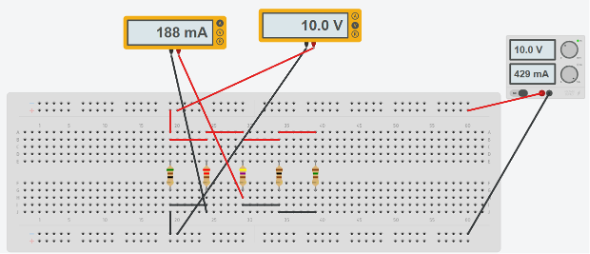
\includegraphics[width=\textwidth]{Figures/1. Content/simulation/paraleloB.png}
      \captionof{figure}{Simulación Conexión en Paralelo en nodo $b$}
      \label{fig: Simulacion Conexion Paralelo B}
    \end{minipage}
    \hfill
    \begin{minipage}{0.45\textwidth}
      \centering
      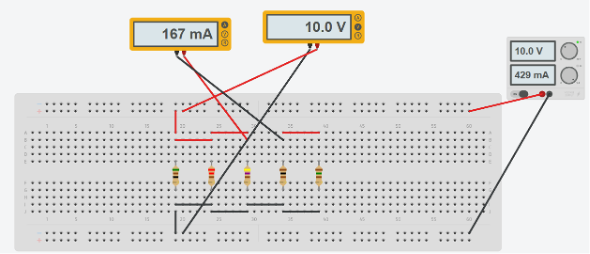
\includegraphics[width=\textwidth]{Figures/1. Content/simulation/paraleloC.png}
      \captionof{figure}{Simulación Conexión en Paralelo en nodo $c$}
      \label{fig: Simulacion Conexion Paralelo C}
    \end{minipage}
    \hfill
    \begin{minipage}{0.45\textwidth}
      \centering
      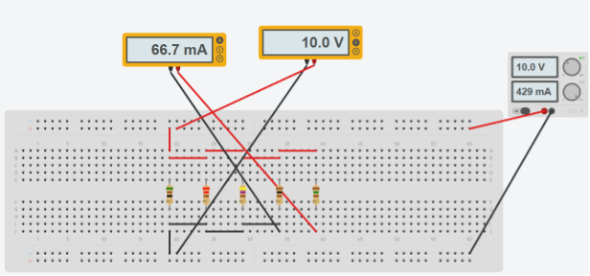
\includegraphics[width=\textwidth]{Figures/1. Content/simulation/paraleloD.png}
      \captionof{figure}{Simulación Conexión en Paralelo en nodo $d$}
      \label{fig: Simulacion Conexion Paralelo D}
    \end{minipage}
    \hfill
    \begin{minipage}{0.45\textwidth}
      \centering
      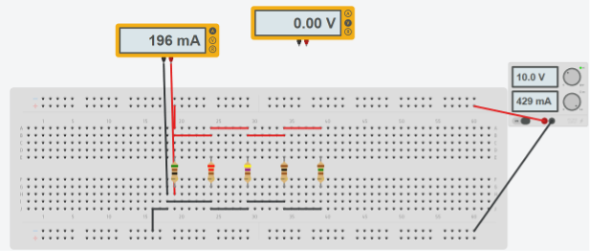
\includegraphics[width=\textwidth]{Figures/1. Content/simulation/paraleloAR1.png}
      \captionof{figure}{Simulación Conexión en Paralelo $I_{R_1}$}
      \label{fig: Simulacion Conexion Paralelo IR1}
    \end{minipage}
    \hfill
    \begin{minipage}{0.45\textwidth}
      \centering
      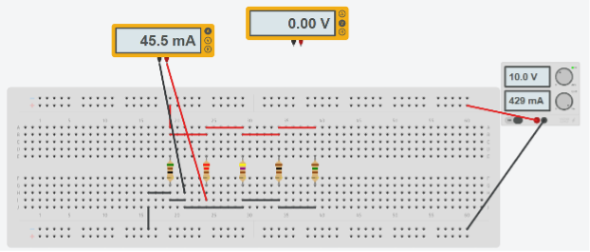
\includegraphics[width=\textwidth]{Figures/1. Content/simulation/paraleloAR2.png}
      \captionof{figure}{Simulación Conexión en Paralelo $I_{R_2}$}
      \label{fig: Simulacion Conexion Paralelo IR2}
    \end{minipage}
    \hfill
    \begin{minipage}{0.45\textwidth}
      \centering
      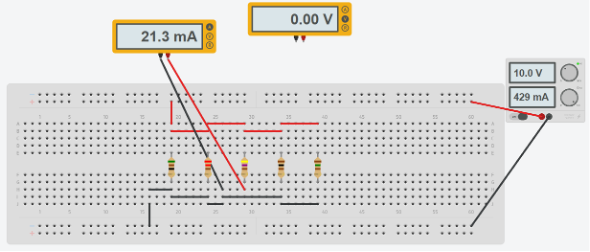
\includegraphics[width=\textwidth]{Figures/1. Content/simulation/paraleloAR3.png}
      \captionof{figure}{Simulación Conexión en Paralelo $I_{R_3}$}
      \label{fig: Simulacion Conexion Paralelo IR3}
    \end{minipage}
    \hfill
    \begin{minipage}{0.45\textwidth}
      \centering
      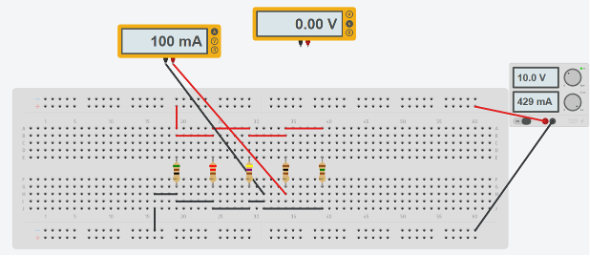
\includegraphics[width=\textwidth]{Figures/1. Content/simulation/paraleloAR4.png}
      \captionof{figure}{Simulación Conexión en Paralelo $I_{R_4}$}
      \label{fig: Simulacion Conexion Paralelo IR4}
    \end{minipage}
    \hfill
    \begin{minipage}{0.45\textwidth}
      \centering
      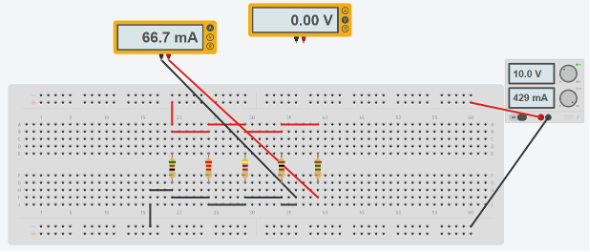
\includegraphics[width=\textwidth]{Figures/1. Content/simulation/paraleloAR5.png}
      \captionof{figure}{Simulación Conexión en Paralelo $I_{R_5}$}
      \label{fig: Simulacion Conexion Paralelo IR5}
    \end{minipage}
\end{figure}


\section{Causas de Error}
Las principales causas de error en este experimento podrían incluir:
\begin{itemize}
    \item Errores de calibración en los instrumentos de medición como amperímetros y voltímetros que podrían haber afectado las mediciones de corriente y voltaje respectivamente.
    \item Resistencias internas de los instrumentos de medición que, aunque diseñadas para minimizar su impacto, pueden introducir pequeñas variaciones en las mediciones.
    \item Variaciones en las resistencias reales respecto a sus valores nominales, lo que podría afectar la distribución de la corriente y el voltaje en el circuito.
    \item Errores en la conexión de los componentes del circuito que podrían haber creado caminos de corriente adicionales o contactos imperfectos.
    \item Influencias ambientales como la temperatura, que puede cambiar las propiedades de los materiales de los componentes, especialmente las resistencias.
\end{itemize}

\section{Conclusiones}
A partir del experimento realizado, se pueden extraer las siguientes conclusiones:
\begin{itemize}
    \item Se confirmó que en un circuito en serie, la corriente es constante a través de cada componente, mientras que la tensión se distribuye entre los componentes en función de su resistencia.
    \item En los circuitos en paralelo, se verificó que la tensión en cada rama es igual a la tensión de la fuente, mientras que la corriente se divide entre las ramas en función de la resistencia de cada una.
    \item Las mediciones experimentales mostraron una buena concordancia con los valores teóricos esperados, aunque con ligeras desviaciones que pueden atribuirse a las causas de error identificadas.
    \item El experimento destacó la importancia de la precisión en la fabricación de los componentes del circuito y la precisión en las técnicas de medición para asegurar la confiabilidad de los resultados experimentales.
    \item Estos resultados refuerzan la comprensión de las leyes fundamentales de los circuitos eléctricos y la importancia de la configuración correcta y el uso adecuado de los instrumentos de medición en prácticas de laboratorio.
\end{itemize}